\chapter[Flujo Ideal y Externo]{Flujo Ideal y Externo}
\section{Ecuación de Euler}

	
	Consideremos un flujo no viscoso ($\mu=0$). La ecuación de Navier-Stokes
	queda entonces como 
	
\begin{equation}
		\Deriv{\vec{u}}{t}=\vec{g}-\frac{1}{\rho}\vec{\nabla}p
\end{equation}
	
	
\begin{equation}
		\dparc{\vec{u}}{t}+\convec\vec{u}=\vec{g}-\frac{1}{\rho}\vec{\nabla}p
\end{equation}
	
	
	La aceleración convectiva se puede escribir en términos da la vorticidad,
	que no es más que el rotacional de la velocidad, $\vec{\omega}=\rot\vec{u}$
	
\begin{equation}
		\convec\vec{u}=\vec{\nabla}\left(\frac{1}{2}u^{2}\right)+\vec{\omega}\times\vec{u}
\end{equation}
	
	
	
	Podemos entonces escribir 
	
\begin{equation}
		\dparc{\vec{u}}{t}+\vec{\nabla}\left(\frac{1}{2}u^{2}\right)+\vec{\omega}\times\vec{u}+\frac{1}{\rho}\vec{\nabla}p-\vec{g}=0
\end{equation}
	
	e integrarlo sobre un cierto camino 
	
\begin{equation}
		\int_{A}^{B}\left[\dparc{\vec{u}}{t}+\vec{\nabla}\left(\frac{1}{2}u^{2}\right)+\vec{\omega}\times\vec{u}+\frac{1}{\rho}\vec{\nabla}p-\vec{g}\right]\cdot\dif\vec{r}=0
\end{equation}
	
	
	Si, por simplicidad, consideramos que el flujo es estacionario, esta
	integral puede ser realizada siempre y cuando $\left(\vec{\omega}\times\vec{u}\right)\cdot\dif\vec{r}=0$.
	Esto ocurre, por ejemplo, si $\vec{u}\cdot\dif\vec{r}=0$. Es decir,
	si el camino es una \textbf{\textcolor{blue}{línea de corriente}}.

	
	En este caso, 
	\[
	\int_{A}^{B}\left[\vec{\nabla}\left(\frac{1}{2}u^{2}\right)+\frac{1}{\rho}\vec{\nabla}p-\vec{g}\right]\cdot\dif\vec{r}=0
	\]
	\[
	\Rightarrow\frac{1}{2}\left(u_{B}^{2}-u_{A}^{2}\right)+g(z_{B}-z_{A})+\int_{A}^{B}\frac{\dif p}{\rho}=0\textrm{ con }\vec{g}=-g\vec{k}
	\]
	
	Esta relación es la conocida \textcolor{blue}{Ecuación de Bernoulli},
	y es válida a lo largo de una línea de corriente. Pero si el flujo
	es irrotacional, es decir, es tal que 
	\[
	\rot\vec{u}=0
	\]
	en todo el dominio, entonces la ecuación de Bernoulli se cumple entre
	dos puntos cualesquiera.

	
	En este caso se cumple que la velocidad, como todo campo vectorial
	conservativo, se puede escribir como gradiente de una función $\phi$
	\[
	\vec{u}=\vec{\nabla}\phi
	\]
	que recibe el nombre de \textbf{\textcolor{red}{potencial de velocidad}}
	y este tipo de flujo se conoce como \textbf{\textcolor{red}{flujo
			potencial}}.
	
	El potencial de velocidad es una función escalar del tiempo y el espacio,
	$\phi(t,x,y,z)$ y se puede definir para cualquier campo de velocidades
	que sea irrotacional.
	
	Las líneas del espacio definidas por $\phi=\text{cte}$ son las \textcolor{blue}{líneas
		de potencial} del flujo.
	
	Para un flujo potencial la ecuación de continuidad se reduce a una
	\textbf{\textcolor{red}{ecuación de Laplace}} 
	\[
	\vec{\nabla}\cdot\vec{u}=0\enskip\Rightarrow\enskip\vec{\nabla}\left(\vec{\nabla}\phi\right)=\nabla^{2}\phi=0\;;\;\dparcsec{\phi}{x}+\dparcsec{\phi}{y}+\dparcsec{\phi}{z}=0
	\]
	

\section{Función de corriente}

	
	Recordemos que, para \textcolor{blue}{un flujo bidimensional}, la
	función de corriente se define como una función $\psi$ tal que $u=\dparc{\psi}{y},v=-\dparc{\psi}{x}$
	de forma que 
	\[
	\dif\psi=\dparc{\psi}{x}\dif x+\dparc{\psi}{y}\dif y=-v\dif x+u\dif y
	\]
	Si $\dif\psi=0$, entonces 
	\[
	\deriv{y}{x}=\frac{v}{u}\enskip\Rightarrow\enskip\psi=\text{cte define las lineas de corriente}
	\]
	Si el flujo es irrotacional 
	\[
	\left(\rot\vec{u}\right)_{z}=\dparc{v}{x}-\dparc{u}{y}=0\enskip\Rightarrow\enskip-\dparcsec{\psi}{x}-\dparcsec{\psi}{y}=0\enskip\Rightarrow\enskip\nabla^{2}\psi=0
	\]
	La función de corriente también cumple la equación de Laplace.

	
	En muchas ocasiones es conveniente (o imprescindible) trabajar en
	coordenadas polares. En estas coordenadas, las relaciones entre la
	velocidad, la función de corriente y el potencial de flujo son 
	\begin{eqnarray}
		u_{r} & = & \dparc{\phi}{r}=\frac{1}{r}\dparc{\psi}{\theta}\\
		u_{\theta} & = & \frac{1}{r}\dparc{\phi}{\theta}=-\dparc{\psi}{r}
	\end{eqnarray}
	y las ecuaciones de Laplace son 
	\begin{eqnarray}
		\frac{1}{r}\dparc{}{r}\left(r\dparc{\psi}{r}\right)+\frac{1}{r^{2}}\dparcsec{\psi}{\theta} & = & 0\\
		\frac{1}{r}\dparc{}{r}\left(r\dparc{\phi}{r}\right)+\frac{1}{r^{2}}\dparcsec{\phi}{\theta} & = & 0
	\end{eqnarray}
	


\section{La ecuación de vorticidad}

	
	Si volvemos a considerar la viscosidad, la ecuación de Navier-Stokes,
	se puede expresar como 
	
\begin{equation}
		\dparc{\vec{u}}{t}+\vec{\nabla}\left(\frac{1}{2}u^{2}\right)+\vec{\omega}\times\vec{u}=-\frac{1}{\rho}\vec{\nabla}p+\vec{g}+\nu\nabla^{2}\vec{u}
\end{equation}
	
	Considerando flujo incompresible y, dado que $\vec{g}=-\nabla gz$,
	obtenemos 
	
\begin{equation}
		\dparc{\vec{u}}{t}+\vec{\omega}\times\vec{u}=-\vec{\nabla}\left[\frac{p}{\rho}+\left(\frac{1}{2}u^{2}\right)+gz\right]+\nu\nabla^{2}\vec{u}
\end{equation}
	
	Si el flujo es estacionario, inviscido e irrotacional,
		recuperamos la ecuación de Bernoulli.

	
	Y ahora hacemos el rotacional de toda esta ecuación, de forma que
	el gradiente desaparece. 
	
\begin{equation}
		\dparc{\vec{\omega}}{t}+\rot\left(\vec{\omega}\times\vec{u}\right)=\nu\nabla^{2}\vec{\omega}
\end{equation}
	
	Esto ya da una información importante: Si el flujo es inviscido,
	y el rotacional es inicialmente cero, se mantendrá nulo de forma indefinida
	
	Podemos escribirlo en forma de transporte, usando la relación de cálculo
	vectorial 
	\[
	\rot\left(\vec{A}\times\vec{B}\right)=\left[\left(\vec{\nabla}\cdot\vec{B}\right)+\left(\vec{B}\cdot\vec{\nabla}\right)\right]\vec{A}-\left[\left(\vec{\nabla}\cdot\vec{A}\right)+\left(\vec{A}\cdot\vec{\nabla}\right)\right]\vec{B}
	\]
	de forma que 
	
\begin{equation}
		\rot\left(\vec{\omega}\times\vec{u}\right)=\left(\vec{u}\cdot\vec{\nabla}\right)\vec{\omega}-\left(\vec{\omega}\cdot\vec{\nabla}\right)\vec{u}
\end{equation}
	
	
	Dado que, para flujo incompresible, $\vec{\nabla}\cdot\vec{u}=\vec{\nabla}\cdot\vec{\omega}=0$,
	la \textcolor{red}{ecuación de la vorticidad} queda como 
	
\begin{equation}
		\dparc{\vec{\omega}}{t}+\left(\vec{u}\cdot\vec{\nabla}\right)\vec{\omega}=\left(\vec{\omega}\cdot\vec{\nabla}\right)\vec{u}+\nu\nabla^{2}\vec{\omega}
\end{equation}
	
	
	\subsection*{Actividad 1:}
		¿ Cómo se simplifica esta expresión para flujo bidimensional? ¿Qué
		conclusiones se pueden extraer en 2D?

	\subsection*{Actividad 2:}
		Expresar la ecuación de vorticidad en términos de la función de corriente


\section{Flujos potenciales elementales}
	
	\begin{itemize}
		\item Dado que las ecuaciones de Laplace son lineales, se puede formar cualquier
		flujo potencial como superposición de varios.
		\item Se consideran tres flujos potenciales elementales a partir de los
		cuales se pueden construir una gran variedad. 
	\end{itemize}
	Estos son:
 \begin{itemize}
 	
\item{Flujo uniforme}
	
	\begin{minipage}[c]{0.6\textwidth}%
		%
		\begin{tabular}{|c|c|}
			\hline 
			coord. cartesianas  & coord. polares \tabularnewline
			\hline 
			$u=U_{\infty}$  & $u_{r}=U_{\infty}\cos\theta$ \tabularnewline
			$v=0$  & $u_{\theta}=-U_{\infty}\sin\theta$ \tabularnewline
			$\psi=U_{\infty}y$  & $\psi=U_{\infty}r\sin\theta$ \tabularnewline
			$\phi=U_{\infty}x$  & $\phi=U_{\infty}r\cos\theta$ \tabularnewline
			\hline 
		\end{tabular}%
	\end{minipage}%
	\begin{minipage}[c]{0.4\textwidth}%
		
\begin{center}
	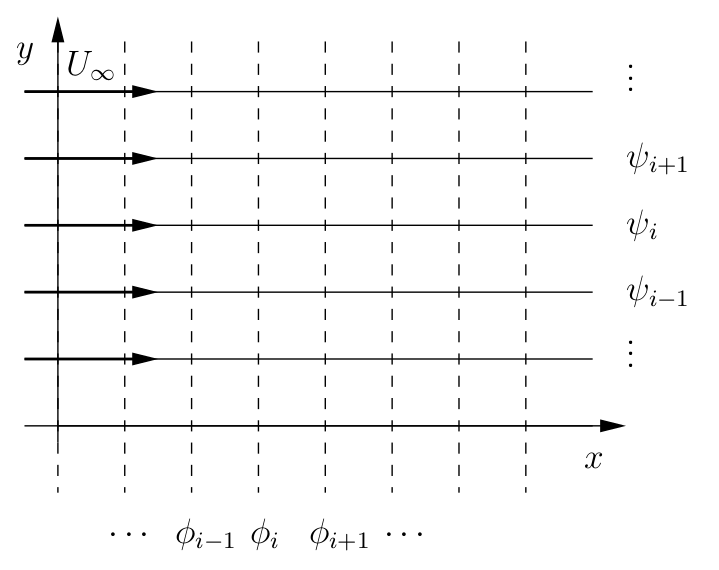
\includegraphics[width=\linewidth]{TeX_files/chapter09-Externo/uniforme}
\end{center}


	\end{minipage}

\item{Fuente o sumidero}
	
	\begin{minipage}[c]{0.6\textwidth}%
		%
		\begin{tabular}{|c|c|}
			\hline 
			coord. cartesianas  & coord. polares \tabularnewline
			\hline 
			$u=m{x}/{(x^{2}+y^{2})}$  & $u_{r}={m}/{r}$ \tabularnewline
			$v=m{y}/{(x^{2}+y^{2})}$  & $u_{\theta}=0$ \tabularnewline
			$\psi=m\arctan({y}/{x})$  & $\psi=m\theta$ \tabularnewline
			$\phi=m\ln\sqrt{x^{2}+y^{2}}$  & $\phi=m\ln r$ \tabularnewline
			\hline 
		\end{tabular}%
	\end{minipage}%
	\begin{minipage}[c]{0.4\textwidth}%
\begin{center}
	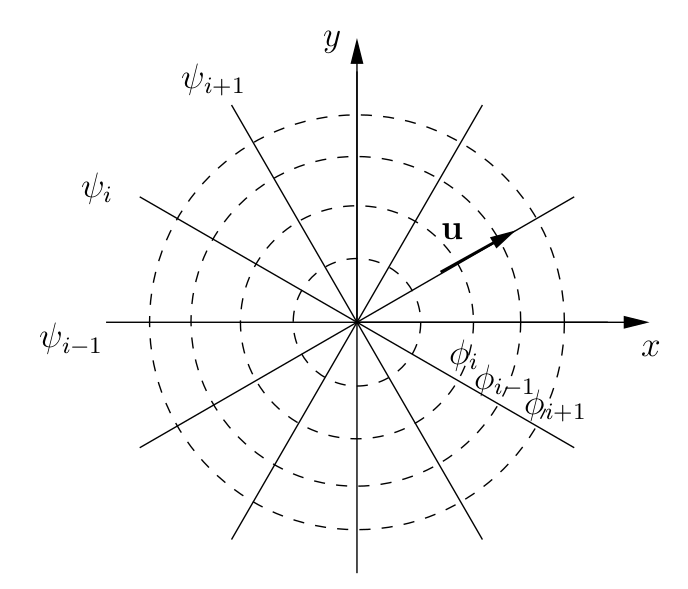
\includegraphics[width=\linewidth]{TeX_files/chapter09-Externo/fuente}
\end{center}
	\end{minipage}

\item{Vórtice o remolino}
	
	\begin{minipage}[c]{0.6\textwidth}%
		%
		\begin{tabular}{|c|c|}
			\hline 
			coord. cartesianas  & coord. polares \tabularnewline
			\hline 
			$u=-K{y}/{(x^{2}+y^{2})}$  & $u_{r}=0$ \tabularnewline
			$v=K{x}/{(x^{2}+y^{2})}$  & $u_{\theta}=K/r$ \tabularnewline
			$\psi=-K\ln\sqrt{x^{2}+y^{2}}$  & $\phi=-K\ln r$ \tabularnewline
			$\phi=K\arctan({y}/{x})$  & $\psi=K\theta$ \tabularnewline
			\hline 
		\end{tabular}%
	\end{minipage}%
	\begin{minipage}[c]{0.4\textwidth}%
\begin{center}
	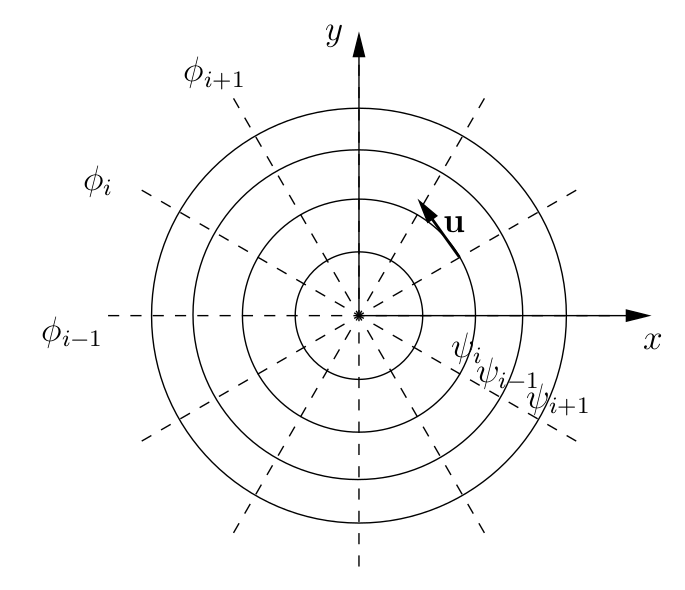
\includegraphics[width=\linewidth]{TeX_files/chapter09-Externo/vortice}
\end{center}
	\end{minipage}
\end{itemize}

\section{Circulación}

	
	El \textcolor{blue}{teorema de Stokes} afirma que para un cierto campo
	vectorial bidimensional $\vec{u}$, la integral sobre una linea cerrada
	es igual a la integral del rotacional del campo sobre la superficie
	que define la linea 
	\[
	\oint_{C}\vec{u}\cdot\dif\vec{r}=\int_{S}\left(\rot\vec{u}\right)\cdot\dif\vec{S}
	\]
	
	En el caso de un campo de velocidades, la integral sobre una linea
	cerrada recibe el nombre de circulación del flujo 
	\[
	\Gamma=\oint_{C}\vec{u}\cdot\dif\vec{r}
	\]
	
	Evidentemente, si el campo es irrotacional, la circulación sobre cualquier
	linea cerrada será nula. Esto es cierto excepto en el caso del vórtice.

	
	\subsection*{Actividad 3:}
		Comprobar que en un vórtice el rotacional es nulo en todos los puntos
		del plano excepto en el origen de coordenadas, donde tiene un valor
		infinito.
		
		En el caso del vórtice, la vorticidad tiene la forma de una delta
		de Dirac (función de valor nulo en todos los puntos excepto en uno,
		en el que tiene valor infinito, y integral finita). El valor de la
		integral de la vorticidad se puede calcular mediante la circulación.

	\subsection*{Actividad 4:}
		Comprobar que la circulación de un vórtice sobre un circulo cualquiera
		que encierra el origen de coordenadas es $\Gamma=2\pi K$.

Ésta circulación es la \textcolor{blue}{fuerza}
		del vórtice. Puede ser positiva o negativa en función de la dirección
		del flujo del vórtice (horario o antihorario).

\subsection{Dos ejemplos de flujos formados como superposición de los tres flujos
		elementales:}
	
	\begin{itemize}

	\item \textcolor{red}{El dipolo}. Formado por una fuente y un sumidero,
	con el mismo valor de $m$, separados una distancia $2a$. 
	\[
	\psi=-m\arctan\frac{2ay}{x^{2}+y^{2}-a^{2}}\quad;\quad\phi=\frac{1}{2}m\ln\frac{(x+a)^{2}+y^{2}}{(x-a)^{2}+y^{2}}
	\]
	\begin{minipage}[c]{0.5\columnwidth}%
		cuando $m\rightarrow\infty$ y $a\rightarrow0$, 
		\[
		\psi=-\dfrac{d}{r}\sin\theta\quad;\quad\phi=\dfrac{d}{r}\cos\theta
		\]
		con $d=ma$%
	\end{minipage}%
	\begin{minipage}[c]{0.45\columnwidth}%
		\begin{center}
			\begin{tikzpicture}[line cap=round,line join=round,>=triangle 45,x=1.0cm,y=1.0cm,scale=2.0]
				\draw[->,color=black] (-1,0) -- (1.03,0) node[below]{$x$};
				%\foreach \x in %{-1,-0.8,-0.6,-0.4,-0.2,0.2,0.4,0.6,0.8,1}
				%\draw[shift={(\x,0)},color=black] %(0pt,2pt) -- (0pt,-2pt) node[below] %{\tiny $\x$};
				\draw[->,color=black] (0,-0.71) -- (0,0.84) node[left]{$y$};
				%\foreach \y in %{-0.6,-0.4,-0.2,0.2,0.4,0.6,0.8}
				%\draw[shift={(0,\y)},color=black] %(2pt,0pt) -- (-2pt,0pt) node[left] %{\tiny $\y$};
				%\draw[color=black] (0pt,-10pt) %node[right] {\footnotesize $0$};
				\clip(-1,-0.71) rectangle (1.03,0.84);
				{
					\draw [line width=1.2pt] (0,-1) circle (1cm);
				}
				{
					\draw [line width=1.2pt] (0,-0.5) circle (0.5cm);
				}
				{
					\draw [line width=1.2pt] (0,-0.67) circle (0.67cm);
				}
				{
					\draw [line width=1.2pt] (0,1) circle (1cm);
				}
				{
					\draw [line width=1.2pt] (0,0.5) circle (0.5cm);
				}
				{
					\draw [line width=1.2pt] (0,0.67) circle (0.67cm);
				}
				{
					\draw [dash pattern=on 1pt off 1pt] (1,0) circle (1cm);
				}
				{
					\draw [dash pattern=on 1pt off 1pt] (0.67,0) circle (0.67cm);
				}
				{
					\draw [dash pattern=on 1pt off 1pt] (0.5,0) circle (0.5cm);
				}
				{
					\draw [dash pattern=on 1pt off 1pt] (2,0) circle (2cm);
				}
				{
					\draw [dash pattern=on 1pt off 1pt] (-2,0) circle (2cm);
				}
				{
					\draw [dash pattern=on 1pt off 1pt] (-1,0) circle (1cm);
				}
				{
					\draw [dash pattern=on 1pt off 1pt] (-0.5,0) circle (0.5cm);
				}
				{
					\draw [dash pattern=on 1pt off 1pt] (-0.67,0) circle (0.67cm);
				}
			\end{tikzpicture}
			\par\end{center}%
	\end{minipage}

	
	 \item \textcolor{red}{El semióvalo de Rankine}. Formado por una fuente (o
	sumidero) y un flujo uniforme. 
	\[
	\psi=U_{\infty}r\sin\theta+m\theta\quad;\quad\phi=U_{\infty}r\cos\theta+m\ln r
	\]
	
\begin{center}
	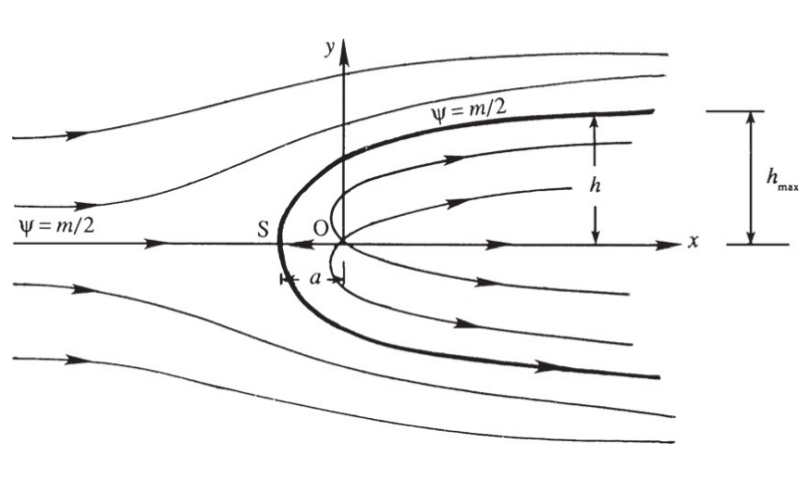
\includegraphics[width=0.7\linewidth]{TeX_files/chapter09-Externo/rankine}
\end{center}

\end{itemize}

\section{Aerodinámica}

	
	Se habla de flujo externo cuando un cuerpo sólido se encuentra completamente
	sumergido en un flujo.
	
	En Flujo Ideal hemos visto las ecuaciones de Euler, cuando no se considera
	la viscosidad, y en flujo potencial cuando, además, el flujo es irrotacional.
	El flujo real se parece más al potencial (irrotacional) cuanto menor
	es el número de Reynolds)
\subsection{Flujo alrededor de un cilindro}
	
	\begin{center}
		\animategraphics[
		controls,scale=0.30
		]{1}{TeX_files/chapter09-Externo/Re}{0}{20}
	\end{center}
	

	
	Pero esto llevaba a la paradoja de D'Alembert, que se resolvía con
	la capa límite.
	
	Los flujo externos reales se estudian conectando ambos modelos: 
	\begin{description}
		\item [{flujo~ideal}] muy lejos del cuerpo, y que determina la forma del
		campo de velocidades y presiones alrededor de él, y 
		\item [{capa~límite}] muy cerca del cuerpo, que determina las fuerzas
		superficiales que actúan sobre él. 
	\end{description}
	En la zona intermedia, ambos modelos deben conectar de forma suave.
	
	La mayor parte de los resultados presentados en el estudio de flujos
	externos son o bien experimentales, o bien numéricos, dada la complejidad
	del problema.


\section{Fuerzas aerodinámicas}

	
	Un flujo externo produce sobre el cuerpo sólido una fuerza $\vec{F}$,
	denominada \textit{aerodinámica}, aunque el fluido no sea necesariamente
	aire.
	
	Esta fuerza se descompone en un sistema de coordenadas definido por
	la dirección del flujo ($x$) y una normal ($z$). La componente en
	la dirección del flujo, $F_{x}$ recibe el nombre de fuerza de arrastre,
	o, simplemente, \textit{arrastre}. En inglés, \textit{drag}, y, por
	esta razón tanto se encuentra escrita como $F_{x}$, como $F_{a}$,
	como $F_{d}$.
	
	La componente en la dirección normal, $F_{z}$, recibe el nombre de
	fuerza de sustentación, o, simplemente, \textit{sustentación}. En
	inglés \textit{lift}, y, por esta razón tanto se encuentra escrita
	como $F_{z}$, como $F_{s}$, como $F_{l}$.
	
	Es importante hacer dos comentarios: 
	\begin{enumerate}
		\item Ni la fuerza de arrastre tiene porqué ser horizontal ni la de sustentación
		vertical 
		\item La velocidad del viento incidente es la \textit{velocidad relativa}
		al cuerpo 
	\end{enumerate}
\begin{center}
	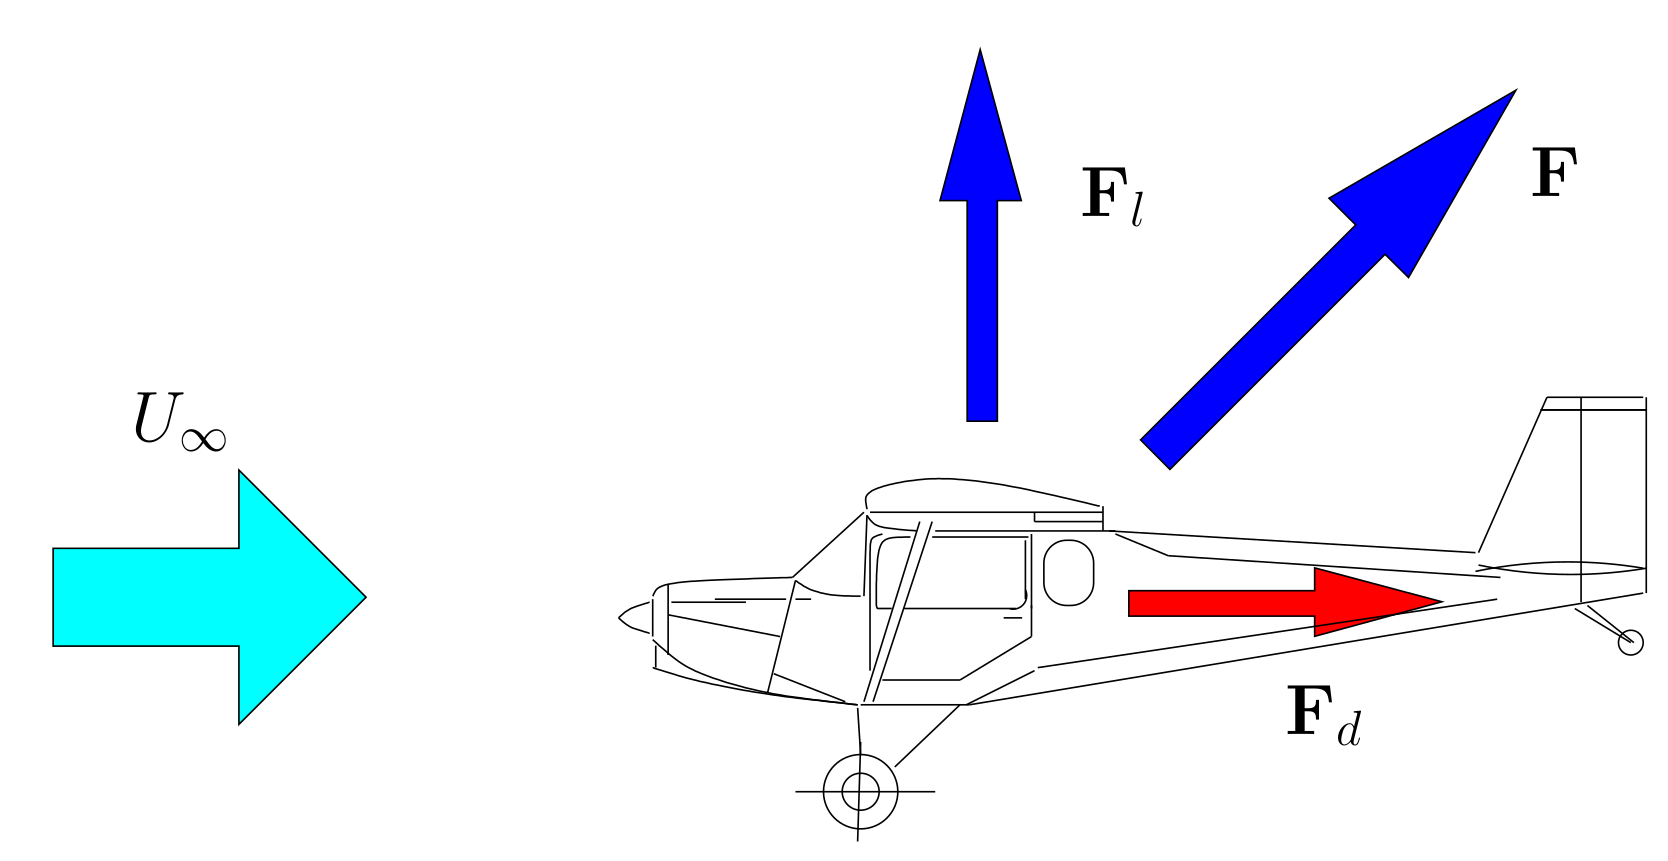
\includegraphics[width=\linewidth]{TeX_files/chapter09-Externo/plane}
\end{center}


\subsection{Arrastre de fricción y de presión}

	
	En el estudio de capa límite vimos cómo actúa la fricción (esfuerzo
	superficial) sobre una placa plana. Pero el arrastre también puede
	ser producido por una diferencia de presión entre la parte anterior
	y posterior del objeto.
	
	Consideremos el ejemplo de una esfera. Si $\Re<1$, no hay prácticamente
	separación, y el arrastre se produce casi por completo por fricción.
	Stokes calculó el valor de este arrastre, 
	
\begin{equation}
		F_{d}=3\pi\mu U_{\infty}D
\end{equation}
	
	
	Sin embargo, para $\Re$ mayores, el desprendimiento del flujo produce
	una zona de baja presión en la estela, y un reflujo en la misma. En
	estas condiciones, el arrastre se debe tanto a la fricción como a
	la presión.


\subsection{Coeficientes aerodinámicos}

	
	Como es habitual, se suelen utilizar magnitudes adimensionales para
	el estudio del flujo externo. La fuerza aerodinámica se compara con
	la presión dinámica del flujo lejano multiplicado por un área de referencia.
	
	El \textcolor{red}{coeficiente de arrastre} es 
	
\begin{equation}
		C_{d}=\dfrac{F_{d}}{\frac{1}{2}\rho U_{\infty}^{2}S_{x}}
\end{equation}
	
	donde $S_{x}$ es la sección proyectada por el cuerpo en la dirección
	del flujo.
	
	Para el \textcolor{red}{coeficiente de sustentación} 
\begin{equation}
		C_{l}=\dfrac{F_{l}}{\frac{1}{2}\rho U_{\infty}^{2}S}
\end{equation}
el área $S$ se define de forma diferente. 

	
	Dado que, para que un cuerpo tenga sustentación tiene que ser, normalmente,
	diseñado para ello (perfiles aerodinámicos), y el área $S_{x}$ varia
	mucho con la orientación del cuerpo, en estos casos, tanto para $C_{d}$
	como para $C_{l}$ se utiliza el área máxima proyectada del cuerpo,
	$S$.
	
	Los coeficientes de arrastre y de sustentación son coeficientes \textit{globales},
	en el sentido que describen el comportamiento del perfil en su totalidad.
	El \textcolor{red}{coeficiente de presión}, $C_{p}$, es un coeficiente
	\textit{local}, definido sobre la superficie del perfil. 
	
\begin{equation}
		C_{p}=\dfrac{p-p_{\infty}}{\frac{1}{2}\rho U_{\infty}^{2}}
\end{equation}
	
	

	
	Aplicando la ley de Stokes para el arrastre viscoso en una esfera,
	el coeficiente de arrastre es 
\begin{equation}
		C_{d}=\dfrac{24}{\Re}
\end{equation}
	
	Pero esto es válido únicamente para $\Re<1$. Para mayores números
	de Reynolds no hay una expresión analítica para $C_{d}$
	
	\begin{minipage}[c]{0.4\textwidth}%
\begin{center}
	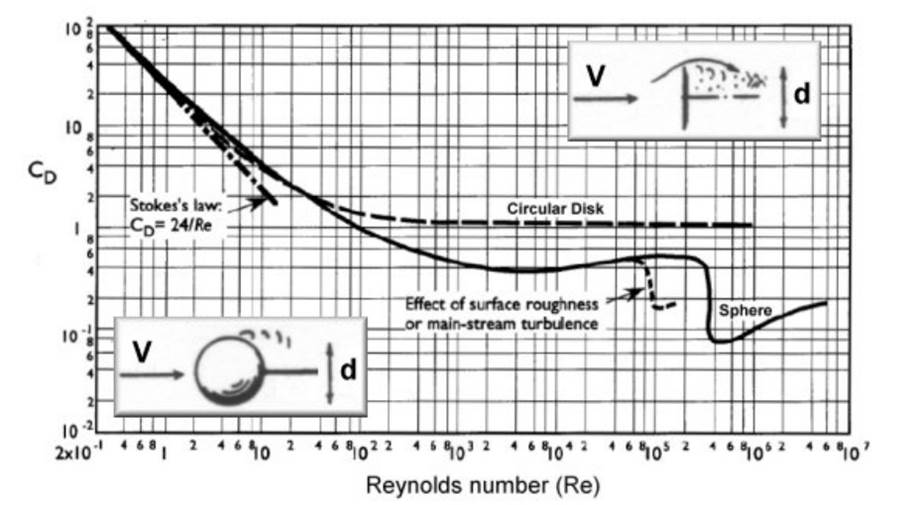
\includegraphics[width=\linewidth]{TeX_files/chapter09-Externo/Cd_esphere}
\end{center}


	\end{minipage} %
	\begin{minipage}[c]{0.5\textwidth}%
		\smallskip{}
		
		Hasta $\Re\approx1000$, el arrastre se produce por combinación de
		la fricción y la presión, debido a la separación de la capa límite.
		A medida que aumenta $\Re$, disminuye la contribución de la fricción,
		de forma que para $\Re\approx1000$ es apenas el 5\% del arrastre
		total.%
	\end{minipage} 
	
	\begin{itemize}
		\item Para $10^{3}<\Re<3\times10^{5}$, la separación del flujo ocurre justo
		en la sección media de la esfera, y la presión en la estela, detrás
		de la esfera es prácticamente constante. Y, por lo tanto, también
		lo es $C_{d}$. La capa límite en la parte delantera de la esfera
		es laminar 
		\item Para $\Re>3\times10^{5}$, la capa límite en la parte delantera es
		turbulenta, y, por lo tanto, se resiste más al desprendimiento. El
		punto de separación se retrasa y esto produce una disminución de $C_{d}$
		debido a la menor sección expuesta a alto gradiente de presiones. 
	\end{itemize}

	
	\begin{minipage}[c]{0.4\textwidth}%
		Esta transición a capa límite turbulenta se puede provocar a menores
		números de Reynolds con la rugosidad de la superficie.
		
		Esta es la razón de la forma rugosa de las pelotas de golf %
	\end{minipage} %
	\begin{minipage}[c]{0.5\textwidth}%
		De Munson\cite{Munson}:
\begin{center}
	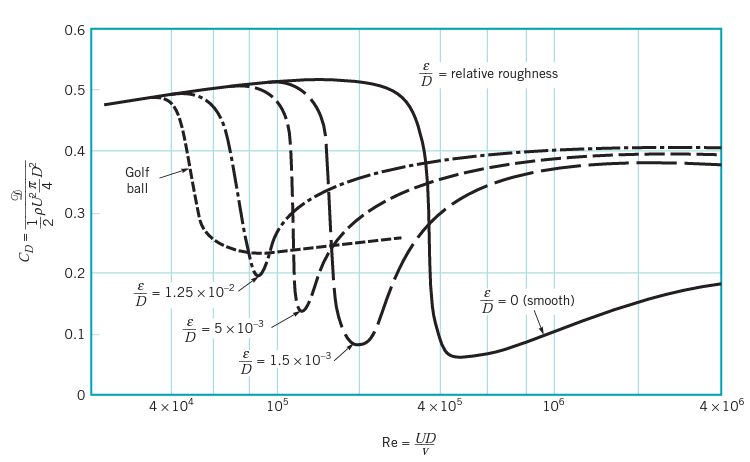
\includegraphics[width=\linewidth]{TeX_files/chapter09-Externo/roughSphere.png}
\end{center}
	\end{minipage}
	
	\smallskip{}
	En el caso de un \textbf{cilindro} (flujo bidimensional) la curva
	$C_{d}-\Re$ es muy parecida, aunque $C_{d}$ es aproximadamente el
	doble.\smallskip{}
	
	\begin{minipage}[c]{0.4\textwidth}%
\begin{center}
	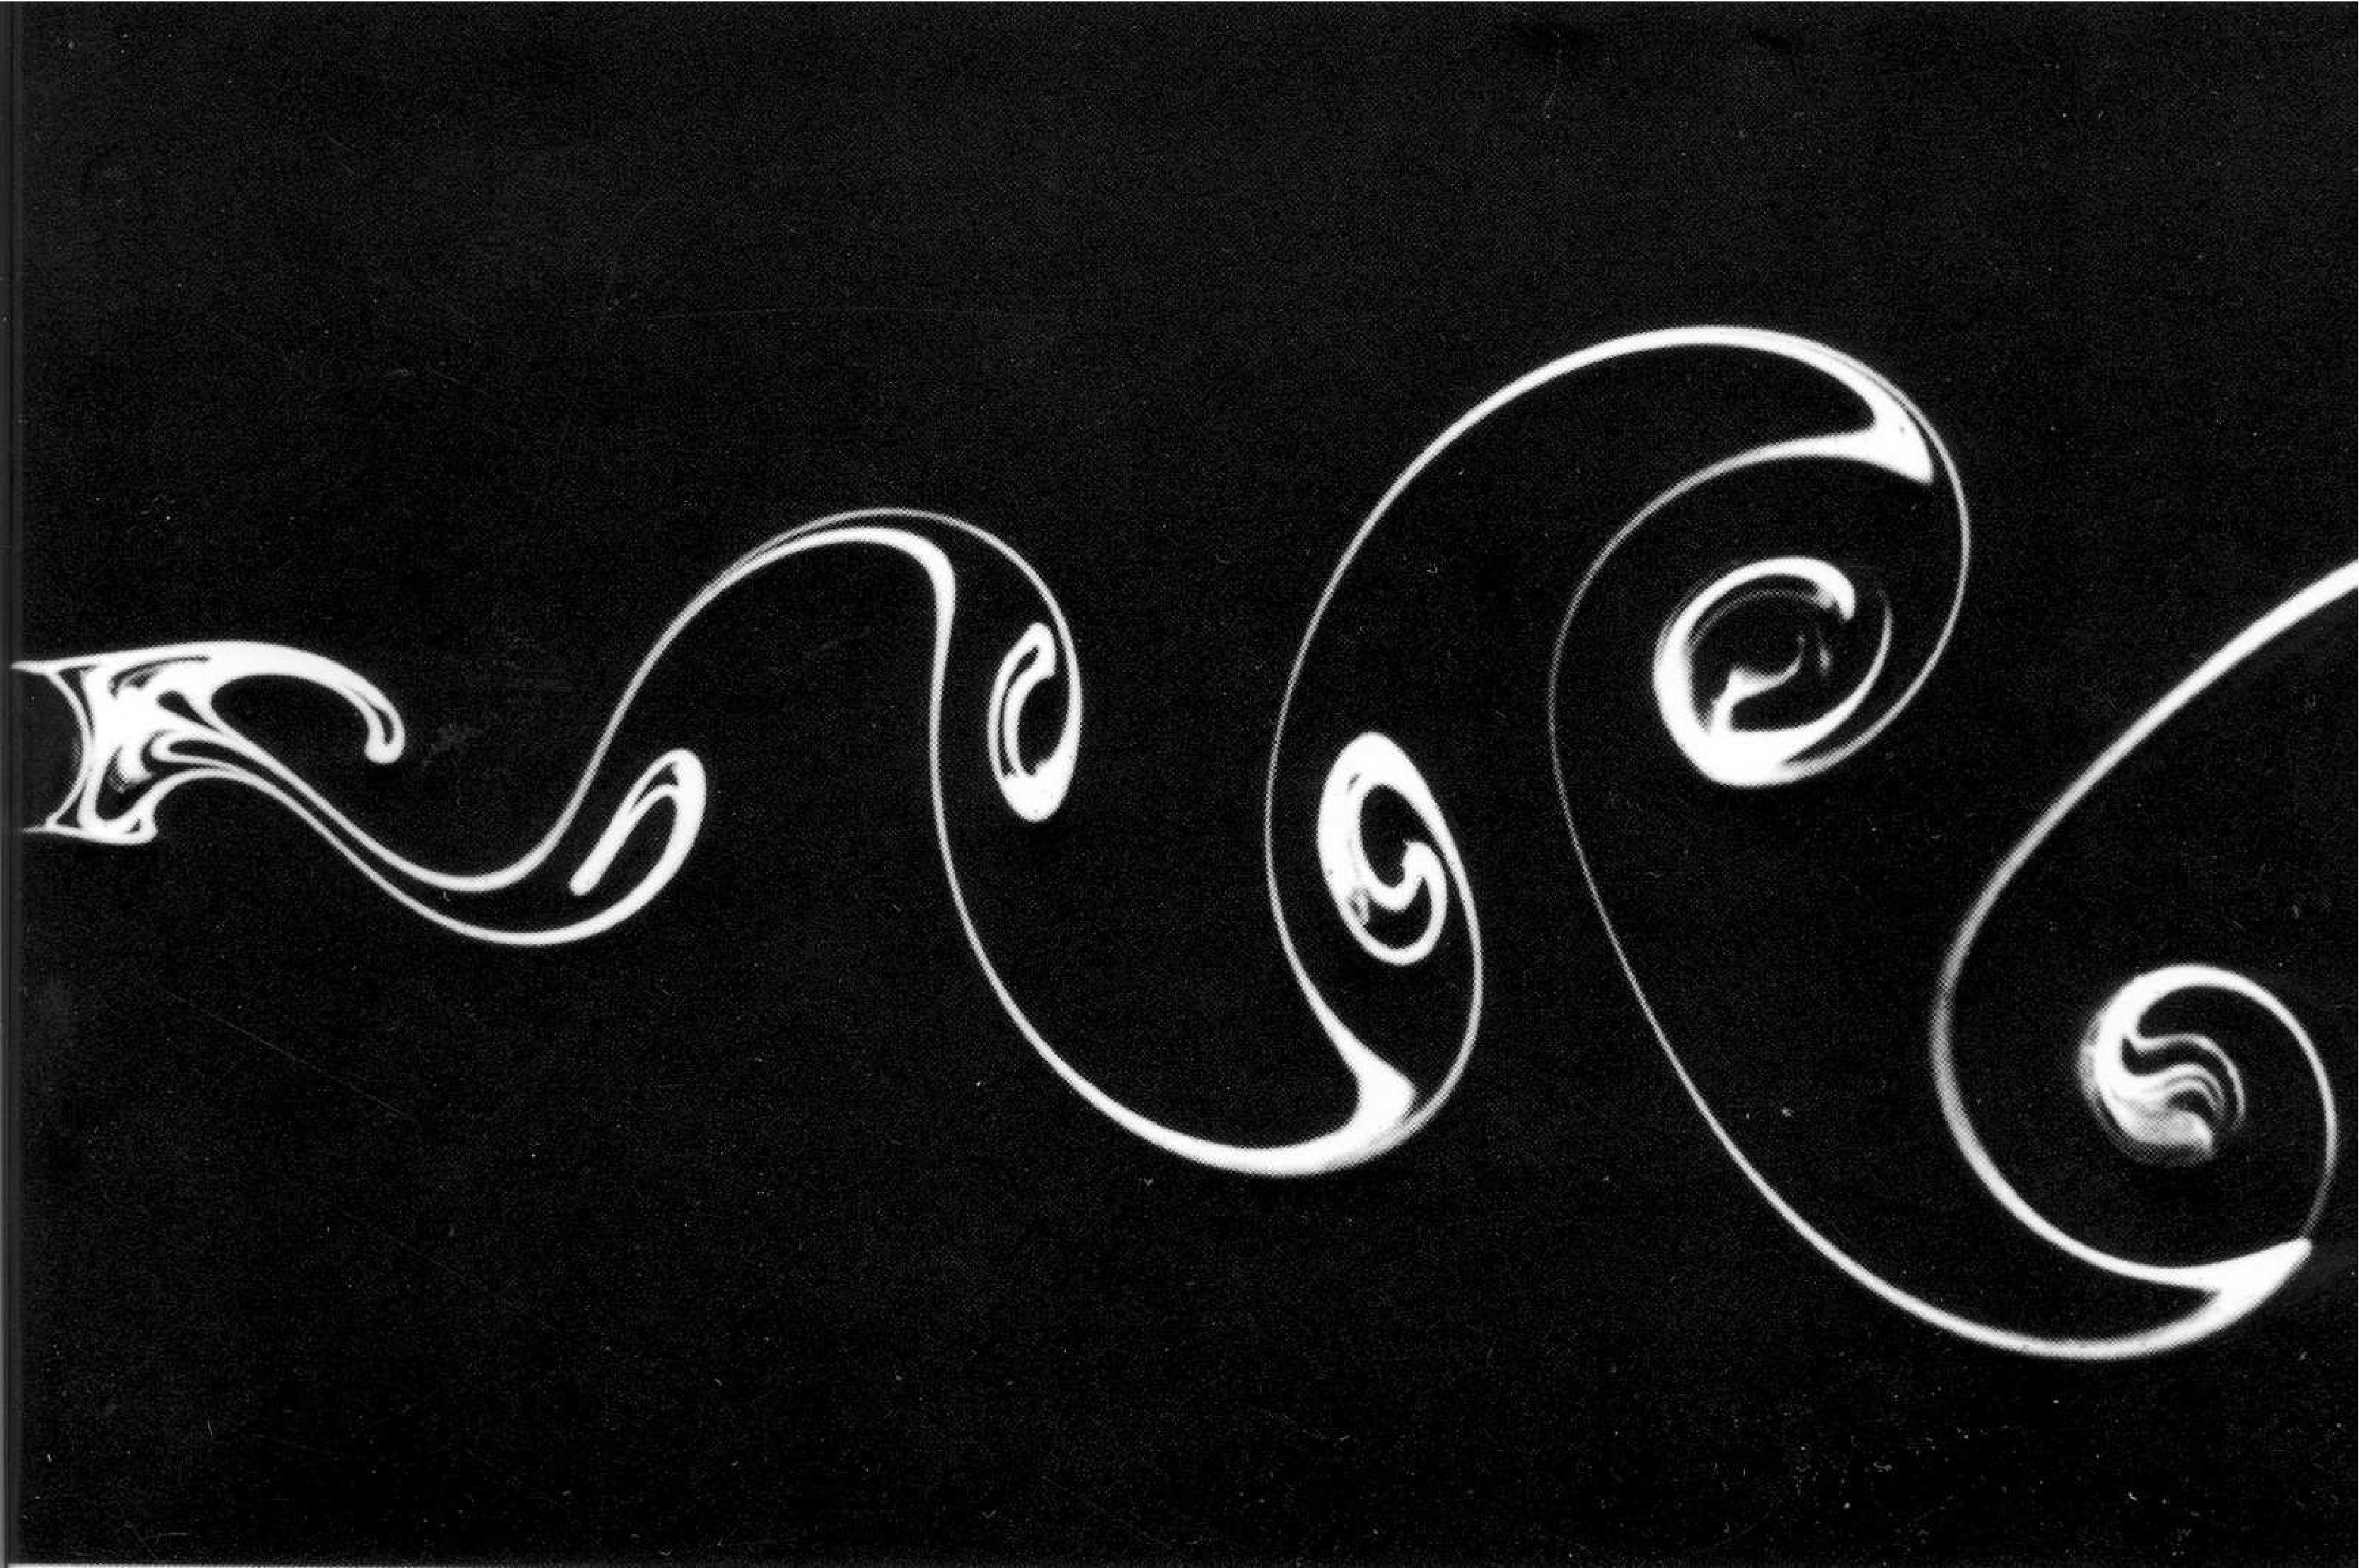
\includegraphics[width=\linewidth]{TeX_files/chapter09-Externo/von_karman}
\end{center}
	\end{minipage} %
	\begin{minipage}[c]{0.58\textwidth}%
		La simetría del cilindro puede provocar la aparición de una serie
		de vórtices uniformemente espaciados en la estela, producidos por
		el desprendimiento alternativo del flujo. Se conoce como estela de
		vórtices o \textit{calle de von Kármán}, y aparece para $60<\Re<5000$. %
	\end{minipage}

	
	Esta estela la responsable de la oscilación de las banderas, del zumbido
	de los cables. Se pueden eleminar con elementos que destruyan la simetría.
	Para $\Re>1000$ el número de Strouhal ($\textrm{St}\equiv\frac{fD}{V_{\infty}}$)
	de esta calle de vórtices es aproximadamente 0,21. 
	
	\begin{center}
		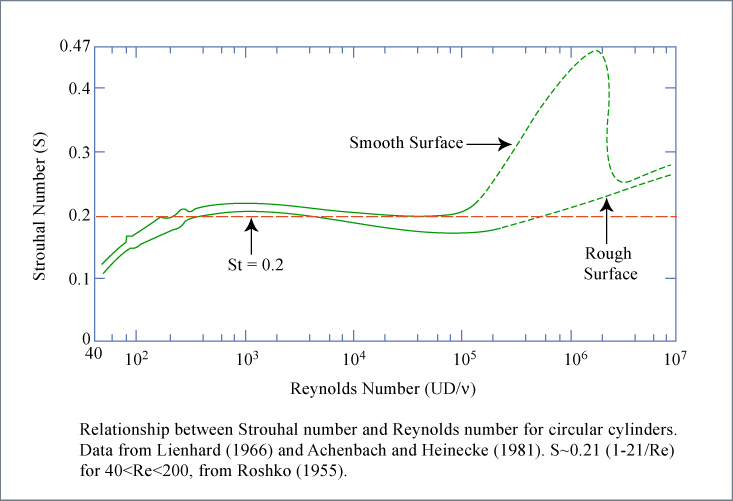
\includegraphics[width=\linewidth]{TeX_files/chapter09-Externo/strouhal-reynolds}
	\end{center}
	
	

	
	\subsection*{Actividad 1:}
		Una chimenea cilíndrica de 1 m de diámetro y 25 metros de alto está
		expuesta a un viento uniforme de 50 km/h en condiciones atmosféricas
		estándar. Los efectos de los extremos se pueden despreciar. 
		
		Estimar el momento de flexión en la base de la chimenea debido a la
		fuerza del viento.
		
		Estimar la frecuencia de los vórtices de von Kármán creados en la
		chimenea.


	

		En esta tabla se presentan algunos $C_{d}$ de cuerpos 2D y 3D, para
		$\Re\gtrsim10^{3}$. Dado que el arrastre se produce mayoritariamente
		por presión, el coeficiente es prácticamente constante.%

\begin{center}
	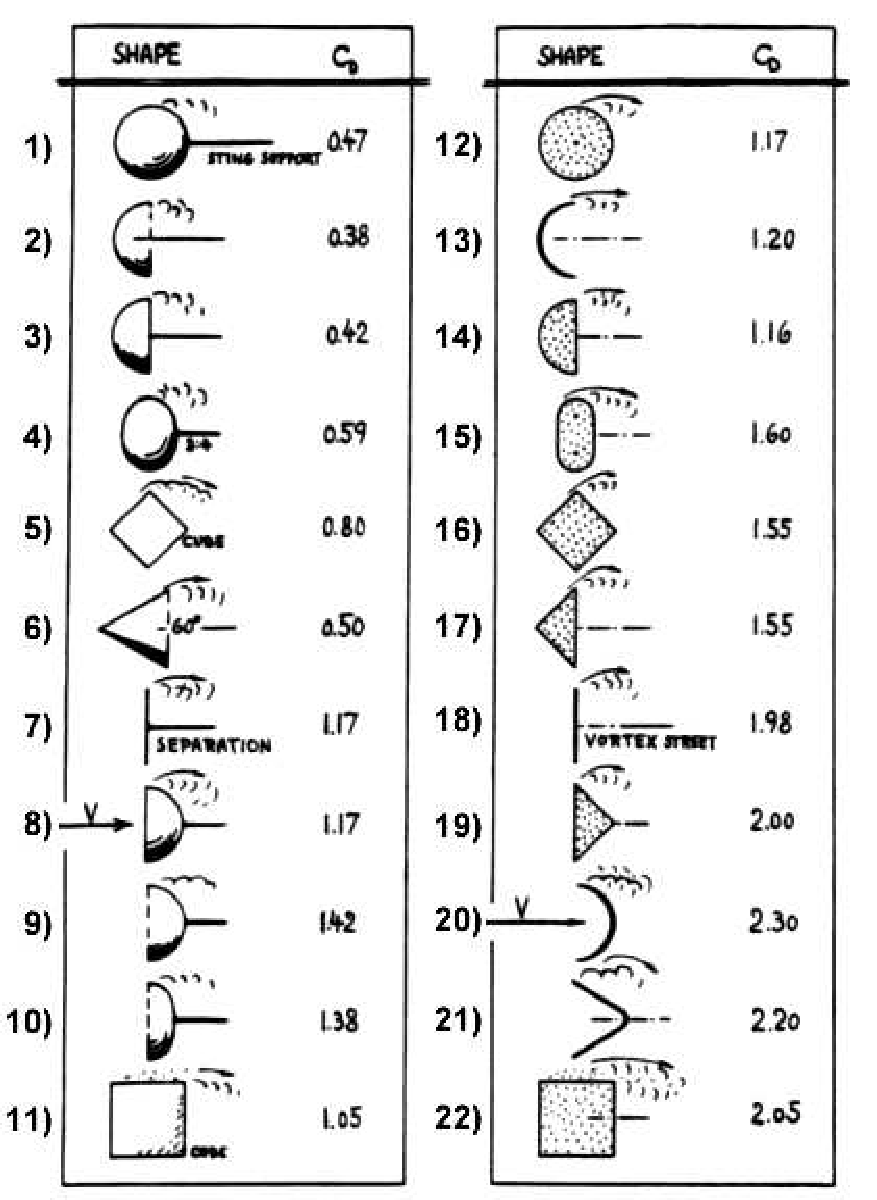
\includegraphics[width=0.6\linewidth]{TeX_files/chapter09-Externo/drag-shapes}
\end{center}


	
	\subsection*{Actividad 2:}
		Un coche de competición, con una masa de 1000 Kg, que circula con
		una velocidad de 350 km/h frena con un paracaidas de 3 m$^{2}$. Estima
		el tiempo y la distancia necesarios para reducir la velocidad a la
		mitad.
		
		Nota: Un paracaídas se puede aproximar a una semiesfera abierta contra
		el viento. 


\subsection{Perfil aerodinámico}

	
	Si se hace un fuselaje a un cilindro en la parte trasera se puede
	evitar el desprendimiento del flujo. Por otro lado, se aumenta el
	área y, por lo tanto, el arrastre por fricción. La forma óptima de
	un perfil aerodinámico es la que minimiza el arrastre total, con una
	gran sustentación.
	
	Definiciones: 
	\begin{itemize}
		\item \textcolor{red}{cuerda}: linea recta que une el borde delantera y
		el borde posterior del perfil. Normalmente se denomina así también
		a su longitud. 
		\item \textcolor{red}{linea media}: linea formada por los puntos medios
		entre curva superior (extradós) y curva inferior (intradós) del perfil,
		según la perpendicular a ella misma. Los perfiles NACA son normalmente
		diseñados combinando una linea media y una distribución de espesor.
		Si la linea media es recta y coincide con la cuerda,se dice que el
		perfil es simétrico. 
	\end{itemize}

	
	Una característica importante de un perfil aerodinámico es el lugar
	de la cuerda en el que se encuentra el espesor máximo. Si este punto
	se retrasa hacia el borde de fuga, el flujo se mantiene laminar gracias
	al gradiente favorable de presión.
	
	Este tipo de perfil  \textit{laminar} tiene muy
	poco arrastre, pero, por otro lado, es más susceptible de entrar en
	pérdida.
	
	Los coeficientes aerodinámicos dependen del ángulo de ataque, que
	es el ángulo que forman la cuerda y la dirección del flujo externo
	no perturbado.
	
	Cuando el perfil está en pérdida, el flujo está completamente desprendido
	en el extradós, y el perfil se hace inestable, bajando $C_{l}$, y
	aumentando considerablemente $C_{d}$. 

\begin{center}
	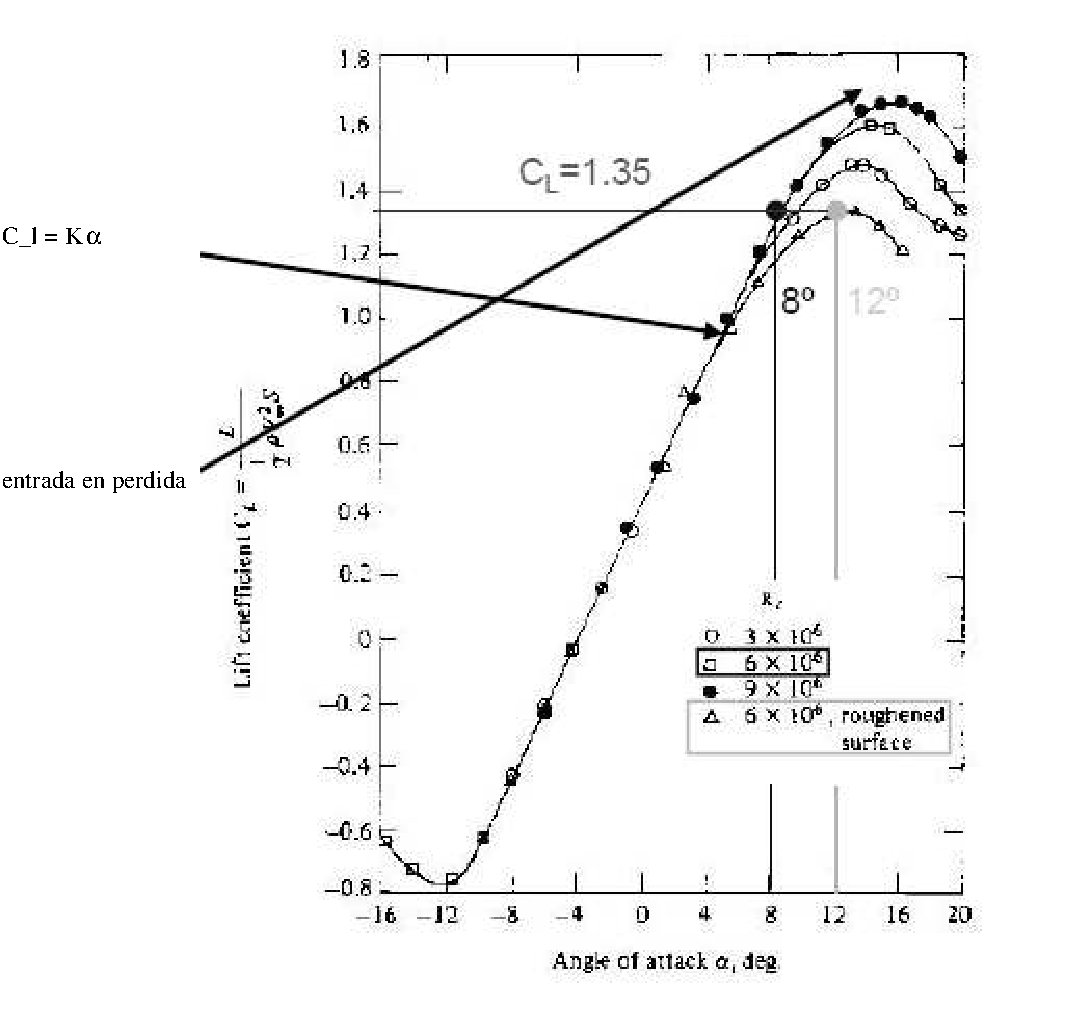
\includegraphics[width=0.6\linewidth]{TeX_files/chapter09-Externo/cl}
\end{center}

\begin{center}
	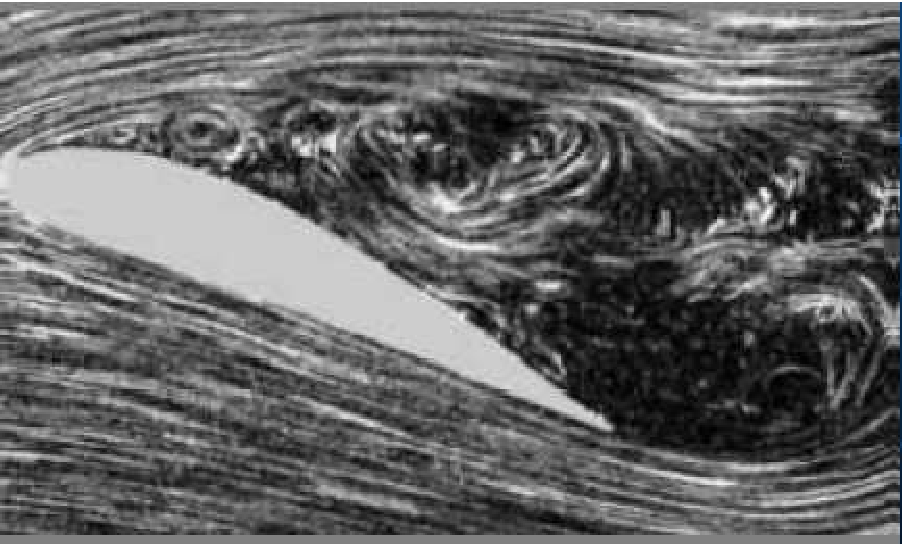
\includegraphics[width=0.7\linewidth]{TeX_files/chapter09-Externo/perdida}
\end{center}
	
